\documentclass[sigconf,anonymous,review]{acmart}
\setcopyright{none}
\settopmatter{printacmref=false}
\acmConference[WWW '27 submission draft]{The Web Conference}{2027}{}
\acmYear{2027}
\acmDOI{}
\acmISBN{}
\usepackage{booktabs,tabularx,multirow,makecell,enumitem,colortbl}
\usepackage{xspace}
\newcommand{\hg}{HybridGuard\xspace}
\newcommand{\full}{\textsc{Full App}\xspace}
\newcommand{\appfp}{\textsc{App177}\xspace}
\newcommand{\browserfp}{\textsc{Browser67}\xspace}
\newcommand{\pairedfp}{\textsc{paired244}\xspace}
\newcommand{\hgstate}[1]{\ensuremath{\mathsf{#1}}}
\begin{document}
\title{HybridGuard: Cross-Layer Fingerprint Consistency for Android Web Environments}
\begin{abstract}
Mobile Web applications observe a device through Android APIs, the WebView host, and JavaScript. These reports overlap, but neither a plausible individual value nor agreement within one surface establishes their integrity. To the best of our knowledge, HybridGuard is the first framework to explicitly formulate mobile fingerprint manipulation detection as consistency checking across Android Native, the WebView host, and in-app Web observations. It separates observed values from unavailable evidence, selects compact detectors under normal-alarm and decision-coverage constraints, and supports a paired external-browser extension. Our controlled App study covers 14 manipulation configurations and uses 891 historical normal-device records for constraint training and evaluation. The full App detector flags 105 of 126 effective modifications (83.3\%) with no alarms on 252 controlled normal records. Removing the historical-normal alarm cap adds only three detections but alarms on every historical normal record. Fixed-check studies show that a device memory reference detects 12 modifications missed by a global threshold, while timezone and host-geometry references distinguish tested normal changes from isolated Web-report modifications. The geometry check remains a standalone study. On 60 paired App--browser positions, adding a cross-endpoint timezone check raises detections from 2/14 to 7/14, entirely through Browser timezone modifications; language modifications remain undetected. These results characterize the capabilities and costs of reference-based checks on development-exposed material, rather than unseen-device generalization or production fraud detection.
\end{abstract}
\begin{CCSXML}
<ccs2012><concept><concept_id>10002978.10003022.10003028</concept_id><concept_desc>Security and privacy~Web application security</concept_desc><concept_significance>500</concept_significance></concept><concept><concept_id>10002978.10002997</concept_id><concept_desc>Security and privacy~Intrusion/anomaly detection and malware mitigation</concept_desc><concept_significance>300</concept_significance></concept></ccs2012>
\end{CCSXML}
\ccsdesc[500]{Security and privacy~Web application security}
\ccsdesc[300]{Security and privacy~Intrusion/anomaly detection and malware mitigation}
\keywords{browser fingerprinting, Android WebView, cross-layer consistency, manipulation detection, missing evidence}
\maketitle
\section{Introduction}
Browser fingerprints summarize properties exposed by a client, including its user agent, language, timezone, display, and graphics environment. Web services use such observations to recognize clients or support authentication decisions, while the same mechanisms create privacy risks~\cite{laperdrix2020browser,alaca2016device,spooren2015harmful}. Their usefulness depends partly on the integrity of the reports: an attacker who controls a reporting surface may change what a service sees without changing the underlying device. Fingerprint spoofing and inconsistent evasive fingerprints are established problems~\cite{liu2022gummy,vastel2018fpscanner,venugopalan2025fpinconsistent}.

Android hybrid applications make this problem distinctive. Web content executes inside a host application that can observe the operating system and configure a WebView. A JavaScript report is therefore one of several partially overlapping accounts of the same environment. An independent system browser can provide another account. This creates an opportunity to ask whether reports are mutually compatible, but also a risk of treating legitimate differences between APIs and containers as manipulation. The Web-security question we study is: \emph{which cross-layer references help detect manipulated mobile Web reports, and what normal-alarm and missing-evidence costs do they introduce?}

A single-field rule illustrates the difficulty. A large reported memory value may exceed a particular device's plausible capacity while remaining below a global threshold. Conversely, a changed timezone may reflect an ordinary system-setting change rather than a manipulated webpage. A screen-height threshold may flag both an effective modification and a harmless layout expansion. The relevant evidence is often a relationship to a contextual reference, not whether an isolated value is unusual. Reference observations are themselves untrusted measurements: consistency cannot attest that all surfaces are truthful.

We develop \hg to study this tradeoff. Its App collector records Android Native, WebView-host, and in-app Web observations under a fixed contract. Checks retain unknown and execution-failure states rather than silently assigning benign values. Offline selection combines admitted conditions into a compact detector subject to normal-alarm and definite-output constraints; online evaluation uses only the current observations required by the frozen detector. An optional pairing path links the App to an independent browser. We distinguish the full App detector, individual mechanism checks, and the retained App-plus-browser extension throughout.

Our evaluation has four parts. First, a controlled benchmark compares the full App detector with four retrained ablations and a small decision tree. Second, historical normal-device records expose the cost of optimizing only controlled detections. Third, memory, timezone, and geometry studies test concrete reference mechanisms against simpler conditions. Fourth, paired observations locate the incremental benefit of a cross-endpoint timezone check. The datasets and model configurations have development-use history; the study is a reproducible characterization of these materials, not a new blind test.

The contributions are:
\begin{itemize}[leftmargin=*,itemsep=1pt,topsep=2pt]
\item An explicit three-view cross-verification framework for Android Native, the WebView host, and in-app Web observations, with state-aware checks that separate contextual references, unavailable evidence, and manipulation alerts.
\item A controlled component analysis: \full flags 105/126 modifications with 0/252 controlled-normal alarms; disabling the historical-normal alarm cap adds three detections but produces alarms on all historical normal records.
\item Mechanism and extension evidence that identifies both benefits and limits: device references recover missed memory modifications and tolerate tested normal changes, while the retained browser extension adds five timezone detections but leaves language modifications unresolved.
\end{itemize}
The findings support evaluating reference checks jointly with normal behavior and evidence availability. They do not establish a universally trusted observation layer, complete manipulation coverage, or a calibrated authentication policy.

\section{Cross-Layer Integrity in Hybrid Web Environments}
\label{sec:setting}
\subsection{Multiple Views of One Execution}
An Android hybrid Web execution provides three complementary, partially overlapping views. Native supplies system and hardware observations; the WebView Host supplies container, configuration, provider, and layout context; App Web exposes JavaScript-visible reports inside that WebView~\cite{android2026webview}. Let $E$ denote the relevant runtime state and container context, beyond a static device model or identifier. We write these observations as $N(E)$, $H(E)$, and $W(E)$ without assuming noiseless, complete, or deterministic API outputs. Associating observations from one execution supports comparison, without implying atomic sampling, trusted collection, or hardware attestation.

The implemented \appfp measurement contract catalogs 84 Native, 26 Host, and 67 App Web fields. An external browser runs a separate Web execution on the same device. \browserfp catalogs 67 fields from that execution; \pairedfp represents linked App--browser observations. These counts describe implementation catalogs, not independent information or the inputs used by every detector.

\subsection{Cross-Layer Consistency as Integrity Evidence}
Integrity here concerns report manipulation; available evidence limits which relations can be assessed. A local Web-report modification can be illustrated as
\[
\begin{aligned}
x_E &= (N(E),H(E),W(E)),\\
x'_E &= (N(E),H(E),W'(E)).
\end{aligned}
\]
Each semantic relation $C_j$ constrains a relevant subset of observations, such as Native--Web or Host--Web. Its interpretation requires an applicability domain, usable operands, and the necessary measurement context. A difference provides evidence only insofar as it violates that measurement constraint.

Local editing may break an applicable relation when other observations still provide distinguishing context: a plausible Web value can then be incompatible with its reference. Some edits remain within compatible ranges. A normal system timezone change may instead move observations together while preserving their relation. Sampling times and implementation differences still limit this interpretation. More views alone do not guarantee a gain; useful evidence depends on informative references and interpretable constraints. This is a mechanism examined empirically, not a necessary-and-sufficient characterization.

\hg evaluates concrete checks using their current required observations. $E$ is explanatory, not an available ground-truth label: the detector neither reconstructs $E$ nor proves that all observations describe a single authentic environment. The notation does not imply access to pre-change baselines, recovery records, or experiment-stage labels. $C_j$ describes compatibility, whereas $r_j(x)$ in Section~\ref{sec:method} denotes a detection condition's state.

The three-view model does not require every relation to use all views or imply a triangle of validated checks. \full combines within-view and cross-view checks; Host geometry remains a separate, unintegrated study; no standalone Native--Host detection rule has been validated.

\subsection{Adversary and Scope of Integrity Claims}
The tested manipulations alter selected resource, browser, locale, display, and graphics reports through controlled tools, browser emulation, or runtime overrides, without necessarily changing the physical device. Only a measured effect at the target surface qualifies as an \emph{effective modification}; operations with no observable effect remain separate.

Native and Host can also be manipulated. A reference left unchanged by a tested intervention is neither a trusted root nor evidence of statistical or administrative independence. Coordinated changes across compared views, collector control, or backend compromise may evade checks; resistance to these capabilities is unproven. Such evasion differs from misses caused by limited implemented relations or observation coverage.

An alarm means an applicable integrity-check condition triggered; it does not confirm fraud, account takeover, malicious intent, or attacker identity. No alert does not establish authenticity. Evaluation units are saved \emph{record positions} or applicable paired positions; repeated operations are not independent devices. Experiment roles and operation records serve evaluation, not prediction.

\subsection{Normal Variation and Missing Evidence}
Normal system timezone, language, orientation, and application-layout changes affect comparability, as do API precision, units, support, and container state. Semantic relations can account for unit conversion, coarse reporting, measurement intervals, and container applicability. Legitimate differences require interpretation within these constraints; they are not automatically violations or unknown outcomes.

Observation availability, a relation among observations, and the detector's final output are distinct. For a selected condition, \hgstate{T} marks a triggered alarm condition; \hgstate{F} means it does not trigger, without certifying authenticity; \hgstate{U} means required evidence is unavailable or insufficient, or the relation is inapplicable. Execution or association failure is recorded separately as \hgstate{FAILED}. An empty model also has a separate status, not an ordinary normal result.

A missing required operand can prevent judging its relation. An unused field's absence does not independently fail the detector, and a check using only some views does not require all three to be complete. Missing evidence is not filled in as normal. Section~\ref{sec:method} explains how \hg implements these conditional relations and evidence states as executable checks and detectors.

\section{HybridGuard}
\label{sec:method}
\begin{figure*}[t]
\centering
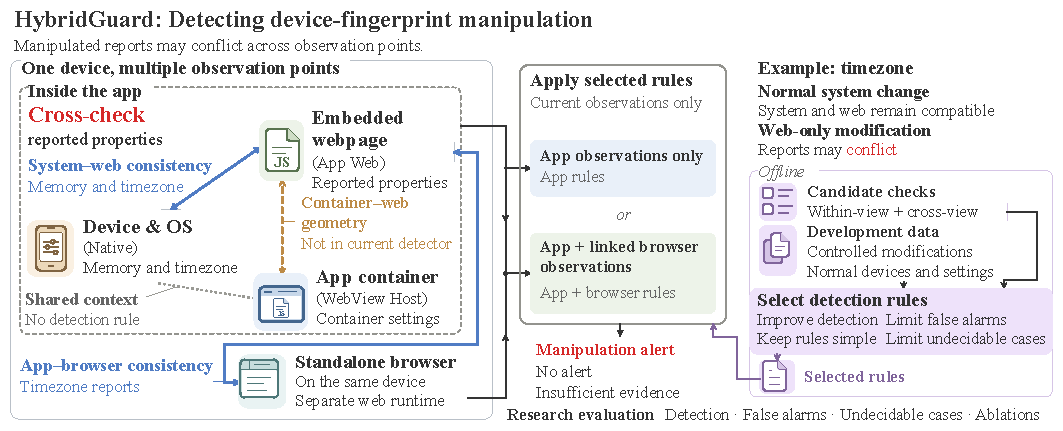
\includegraphics[width=\textwidth]{figures/overview.pdf}
\caption{HybridGuard uses complementary observations from the same device to check fingerprint reports. Offline selection constrains normal alarms and definite-output coverage; frozen detectors consume current App observations or linked App--browser observations. Solid comparison edges denote detector relations. Host--Web geometry is a separate study; the dotted Native--Host edge supplies context only. No surface is trusted ground truth. No alert does not establish safety, and execution failures are recorded separately.}
\Description{Android Native, WebView host, and App Web observations form a triangle. An external browser joins through a pairing step. Offline constrained selection supplies detectors, whose outputs are alert, no alert, or insufficient evidence. A timezone example contrasts a normal system change with a webpage-only modification.}
\label{fig:overview}
\end{figure*}

\subsection{Collection and State-Aware Checks}
Figure~\ref{fig:overview} separates measurement, offline selection, and current-record evaluation. Each field carries a value and an observation status. Normalization handles units and schema versions before a check executes; unsupported, missing, or unparsable operands remain unavailable. Original records, receipts, and pairing metadata support source attribution. A paired view requires two linked observations; an incomplete browser capture leaves an App-only record rather than a fabricated browser vector. Pair identifiers, experiment labels, environment names, and stage metadata are excluded from prediction inputs.

A check is a predicate together with its prerequisites and interpretation. Candidate conditions include single-field thresholds, relations within the App Web view, and Native--Web references. A reference is not an instruction to require exact equality: measurements may be bucketed, unit-converted, or tied to a collection interval. Documentation informs these interpretations, while project predicates and tolerances remain research choices rather than official attack rules.

Let $r_j(x)\in\{\hgstate{T},\hgstate{F},\hgstate{U},\hgstate{FAILED}\}$ be the state of a selected condition on current observation $x$. The detector is an OR of selected singleton conditions. After checking selected-input validity, any execution or binding failure yields \hgstate{FAILED}; otherwise any \hgstate{T} yields an alert, all \hgstate{F} yields no alert, and the remaining cases yield \hgstate{U}. An empty selected set has its own status. Thus a known violation can establish an alert despite another unknown condition, whereas unknown evidence cannot establish a definite no-alert result. Unselected fields do not independently cause failure.

\subsection{Device References}
\paragraph{Memory.}
The memory reference tests whether a positive Web-reported memory value exceeds a coarse upper envelope of observed Native memory:
\begin{equation}
 r_{\mathrm{mem}}(x) = \big[m_{\mathrm{web}}>2^{\lceil\log_2 m_{\mathrm{native}}\rceil}\big].
\label{eq:memory}
\end{equation}
Both operands are expressed in GiB, and validity checks include a Native value of at least 0.25 GiB. The envelope accommodates coarse reporting instead of demanding physical-memory equality. It targets upward violations; a smaller or coordinated plausible report can evade it. We compare it with the fixed condition $m_{\mathrm{web}}>8$ in a separate mechanism study.

\paragraph{Timezone.}
The Native timezone reference derives the effective offset from the device's IANA timezone and its collection interval, using the fixed timezone database 2026c. It compares this offset with the Web \texttt{getTimezoneOffset} value after reversing the UTC-offset sign convention. It compares effective offsets, not timezone-name strings. An ambiguous transition interval or unusable prerequisite yields unknown; zero and minus one are not automatically missing sentinels. This permits an ordinary system timezone change when both observations move consistently, while exposing a Web-only override that does not match the Native reference.

\paragraph{Host geometry.}
A separate check compares visual-viewport geometry with a host measurement of the containing View. For either axis, let $P$ be the CSS visual-viewport size multiplied by device-pixel ratio and visual-viewport scale, and let $H$ be the host View size less its own padding. The check alerts if $P>H+\epsilon$, with $\epsilon=2+4\cdot2^{-23}\max(|P|,|H|,1)$ pixels. Snapshot binding and host-before/after stability are prerequisites. The implemented domain also requires an attached, visible host View, zero padding, and an identity View transform; observations outside that domain yield unknown. This fixed engineering tolerance is not a platform guarantee. The condition is evaluated as a specialist mechanism and is \emph{not} part of \full.

\subsection{Constrained Detector Selection}
The App pool contains 50 base templates and three fixed relations, expanded using the training-side encoder and admissible polarities. The full pool has 65, 65, and 56 expanded atoms across the three model configurations. A candidate must be sufficiently assessable on historical normal training data; absence of a comparable field is not resolved by assuming that the condition is false.

For a selected set $S$, the sparse stage maximizes the heuristic objective
\begin{equation}
 J(S)=\frac{1}{K}\sum_{k=1}^{K}\overline{d}_k(S)-0.005\,C(S),
\label{eq:selection}
\end{equation}
where $K=14$, $\overline{d}_k$ averages detection over training environments and then effective modification positions within configuration $k$, and $C$ counts clauses plus literal occurrences. Selection uses greedy improving additions, retains the best feasible prefix, and performs a backward-pruning pass; it does not guarantee a global optimum.

Feasibility limits a detector to eight singleton OR clauses, complexity 16, and two clauses per registered family, without opposite polarities of the same atom. Separate training-normal alarm budgets are $\lfloor0.05\cdot168\rfloor=8$ for controlled records and $\lfloor0.05\cdot630\rfloor=31$ for historical cloud-device records. Candidate assessability and final definite-output coverage on the latter must each reach 90\%; controlled coverage is constrained per phase at 80\%. Fitting disallows execution failures and uses a 60-second deadline per fit.

The subsequent retention stage starts from that configuration's sparse solution. It can add semantic diversity without losing training detections, or replace a same-group condition with a registered higher-quality alternative under per-record nonregression checks. It does not continue optimizing Equation~\ref{eq:selection}. We evaluate the saved retention outputs consistently, rather than choosing a stage separately for each result cell. The resulting detector is frozen before its designated evaluations.

\subsection{Paired Browser Extension}
The retained paired detector adds a cross-endpoint timezone condition, C1, to the frozen App detector. C1 alerts when the linked App Web and external-browser offsets are unequal. Both are finite numeric Web offsets with the same sign convention; zero and minus one are valid. C1 has no timestamp gate, unlike the interval-aware Native timezone reference. Missing or inapplicable evidence remains unknown under the same state-aware combination. The extension selection compared the empty set, C1, a language condition C2, and their combination, with separate normal-alarm budgets of 31/630 MTC training records, 0/12 pilot normals, and 1/34 matched normals, plus 90\% definite-output coverage. C2 alarms on two matched normal preference changes, and the two-condition combination provides only 566/630 definite MTC training outputs; neither meets the frozen constraints. This offers a second endpoint for testing a mismatch; it does not establish which endpoint is truthful or make language differences suspicious by definition. The extension is evaluated separately from the App benchmark because the original App positions do not have contemporaneous external-browser counterparts.

\section{Evaluation}
\label{sec:eval}
We ask four questions: which modifications are detected and which components matter (RQ1); what cost is hidden by controlled-normal results (RQ2); how contextual references change individual checks (RQ3); and where an external browser adds capability (RQ4).

\subsection{Materials and Protocol}
\paragraph{Controlled App benchmark.}
The benchmark contains 378 positions: 14 modification configurations, three repetitions, three Android emulator environments (API 29, 30, and 36 with SwiftShader), and three stages per run. Admitted runs contain a normal pre-position, an effective modification, and a confirmed normal post-position. This gives 126 effective modifications and 252 normal records. The normal post-position is an evaluation/control record, not an input available to an earlier prediction. Three leave-one-environment-out configurations each use 252 training positions (84 modified, 168 normal) and 126 held-out positions (42 modified, 84 normal). We aggregate the disjoint held-out positions once. Development exposure to these environments and recipes means this partition is not evidence of unseen-tool or independent physical-device generalization.

\paragraph{Historical normal records.}
The mobile test-cloud (MTC) material comprises 891 representative records: 630 discovery records for constraints and tree training, 144 historical development records, and 117 historically reserved evaluation records. Representatives are manufacturer/model/Android-release combinations, not 891 independent physical devices; model families and known installation/session associations constrain grouping. The last two sets are reported separately. Each frozen model is applied to the same records; three model outputs do not triple the sample size. ``Normal'' means no study-defined target manipulation, not an attestation that a cloud device has no automation or debugging software.

\paragraph{Specialist and paired material.}
The memory study has 18 effective modifications and 48 normal records, plus six operations with no observable effect. The timezone study has six modifications and 30 normal records; six normal system changes are a subset of the 30. The screen study has six modifications and 66 normal records, including six normal layout expansions. The App--browser language/timezone material contains 60 paired positions: 14 effective modifications and 46 normal records, from an 18-position pilot and a 42-position matched batch. Normal records total $12+34$, not just the matched subset. These materials have development-use history and distinct roles. We do not add their denominators to produce an overall accuracy or an independent population sample.

\paragraph{Methods.}
\full denotes the saved App retention detector. Four ablations are retrained from their own sparse stage: remove the MTC alarm cap, use App-Web-only candidates, remove the memory reference, or remove the timezone reference. Removing the MTC cap raises its allowance to 630, while retaining MTC data, assessability and coverage constraints, and the controlled-normal budget. Web-only removes Native dependencies, so it changes available information as well as the relationships. The host-geometry specialist and Browser C1 are outside this pool.

The App tree uses the same fold-specific admitted candidate representation, with separate true/false/unknown indicators, maximum depth three, minimum leaf size two, Gini splitting, and a fixed random seed. Training weight is one half for effective modifications, one quarter for controlled normals, and one quarter for MTC normals; modification weight is balanced across configurations. This is a fixed small-capacity reference, not the performance ceiling of machine learning or a classifier over all raw App fields. Rule rows use the saved \texttt{RETENTION} stage and tree rows the saved \texttt{FITTED} stage.

\paragraph{Measures and reporting.}
A detection is an alert on an effective modification; a normal alarm is an alert on a normal record. We retain no-alert, unknown, failed, and empty-model counts. Unknown records stay in denominators rather than being counted as benign. Percentages are descriptive ratios for the stated cohort; we do not estimate population recall, claim significance from repeated configurations, or invent confidence intervals from dependent positions. The tables transcribe frozen results; assembling this draft involved no new collection, fitting, selection, prediction, or timing.

\subsection{RQ1: App Detection and Components}
% English, editable adaptation of 01_app_contribution_compact (2026-10-16).
\begin{table*}[t]
  \caption{App-side detection and component comparisons. Cells give detections out of nine effective modifications per original configuration; parentheses give differences from Full App. Fourteen configurations are grouped only when their complete six-method state-count vectors agree. Adjacent equal results are merged. Group sizes retain the original weighting.}
  \label{tab:app}
  \centering
  \small
  \definecolor{HGappSame}{RGB}{242,244,246}
  \definecolor{HGappLess}{RGB}{247,231,228}
  \definecolor{HGappMore}{RGB}{227,242,235}
  \setlength{\tabcolsep}{4pt}
  \renewcommand{\arraystretch}{1.12}
  \begin{tabularx}{\textwidth}{@{}l c *{6}{>{\centering\arraybackslash}X}@{}}
    \toprule
    Modification group & \makecell{Group\\size} & \makecell{Full\\App} & \makecell{No MTC\\alarm cap} & \makecell{App Web\\only} & \makecell{No memory\\relation} & \makecell{No timezone\\relation} & \makecell{App\\tree} \\
    \midrule
    CPU + memory & 1 & \multicolumn{2}{>{\columncolor{HGappSame}}c}{9} & \multicolumn{2}{>{\columncolor{HGappLess}}c}{$0\;(-9)$} & \cellcolor{HGappSame}9 & \cellcolor{HGappLess}$0\;(-9)$ \\
    \addlinespace[2pt]
    Screen metrics & 1 & \cellcolor{HGappSame}6 & \cellcolor{HGappMore}$9\;(+3)$ & \multicolumn{3}{>{\columncolor{HGappSame}}c}{6} & \cellcolor{HGappLess}$0\;(-6)$ \\
    \addlinespace[2pt]
    Timezone; plugins/MIME & 2 & \multicolumn{5}{>{\columncolor{HGappSame}}c}{9} & \cellcolor{HGappLess}$0\;(-9)$ \\
    \addlinespace[2pt]
    Shared detections$^{\dagger}$ & 8 & \multicolumn{6}{>{\columncolor{HGappSame}}c}{9 (all detected)} \\
    \addlinespace[2pt]
    Webdriver; WebGL IDs & 2 & \multicolumn{6}{>{\columncolor{HGappSame}}c}{0 (all missed)} \\
    \midrule
    Total detections & 14 & 105/126 & 108/126 & 96/126 & 96/126 & 105/126 & 72/126 \\
    \bottomrule
  \end{tabularx}
  \par\smallskip
  \begin{minipage}{\textwidth}\footnotesize
  Gray, green and red indicate equal, more and fewer detections than Full App, respectively; colors do not rank overall method quality.
  $^{\dagger}$Playwright, Puppeteer, CDP multi-field and Stealth presets; platform, UA, UA + platform and language-list modifications.
  All methods have 0/252 controlled-normal alarms; unknown, failed and empty-model counts are zero.
  Rules use saved \textsc{retention} results and the tree uses \textsc{fitted} results. The extra three screen detections without the cap have a separate normal-record cost (Table~\ref{tab:cap}).
  \end{minipage}
\end{table*}

\full detects 105/126 modifications (83.3\%). It produces no alarms on the 252 controlled normal records. Table~\ref{tab:app} compresses the 14 configurations into five groups without dropping configurations: group membership requires matching complete outcome-count vectors across all six methods. Counts within a row are per original configuration, and the group-size column preserves the weighting. These are count equivalences, not claims of identical individual outputs across recipes.

The resource modification accounts for the nine detections lost by Web-only and by removing the memory reference: both fall to 96/126. The small tree detects 72/126. Its additional misses include the tested timezone and plugin/MIME modifications as well as resource and screen modifications. This comparison identifies the behavior of the fixed representation and capacity; it does not show that rules generally outperform learned classifiers.

All methods miss the nine webdriver-only and nine WebGL-identifier modifications. In the current historical-data-compatible pool, raw WebGL unavailability and loss of the original webdriver-false semantics prevent corresponding candidates from meeting assessability requirements. The result is a coverage limit of the admitted representation, not proof that these modifications are intrinsically undetectable.

Removing the MTC alarm cap increases screen detections from six to nine and the total to 108/126. Removing the timezone reference leaves the total at 105/126 because an absolute offset condition substitutes on this benchmark. Neither observation is enough to choose a method: the first requires inspecting normal-record costs, and the second requires normal-setting changes.

\subsection{RQ2: The Cost of Removing Normal Constraints}
% English, editable adaptation of 03_normal_constraint_table (2026-10-16).
\begin{table*}[t]
  \caption{Normal-record outcomes with and without the MTC alarm cap. Removing the cap makes every record in both historical evaluation cohorts trigger an alarm, while controlled detections increase only from 105/126 to 108/126. Both methods still have 0/252 controlled-normal alarms. Counts are records, with unknown outcomes reported separately.}
  \label{tab:cap}
  \centering
  \small
  \setlength{\tabcolsep}{7pt}
  \renewcommand{\arraystretch}{1.1}
  \begin{tabular*}{\textwidth}{@{\extracolsep{\fill}}l c c c c c c c@{}}
    \toprule
    \multirow{2}{*}{Historical cohort} & \multirow{2}{*}{\makecell{Model\\configuration}} & \multicolumn{3}{c}{With cap (Full App)} & \multicolumn{3}{c}{Without cap} \\
    \cmidrule(lr){3-5}\cmidrule(l){6-8}
    & & Alarm & No alarm & Unknown & Alarm & No alarm & Unknown \\
    \midrule
    \multirow{2}{*}{Evaluation ($N=144$)} & 01/02 & \textbf{1} & 135 & 8 & \multirow{2}{*}{\textbf{144}} & \multirow{2}{*}{0} & \multirow{2}{*}{0} \\
    & 03 & \textbf{0} & 136 & 8 & & & \\
    \addlinespace
    \multirow{2}{*}{Reserved ($N=117$)} & 01/02 & \textbf{1} & 110 & 6 & \multirow{2}{*}{\textbf{117}} & \multirow{2}{*}{0} & \multirow{2}{*}{0} \\
    & 03 & \textbf{0} & 111 & 6 & & & \\
    \bottomrule
  \end{tabular*}
  \par\smallskip
  \begin{minipage}{\textwidth}\footnotesize
  Equal counts are merged for display; each configuration uses the same records, so denominators are not pooled. Failed and empty-model counts are zero.
  The separate 630 constraint-training records yield 6/6/0 alarms and 51 unknowns per capped configuration (01/02/03), versus 630 alarms and no unknowns without the cap.
  These historical cohorts are not a new blind evaluation.
  \end{minipage}
\end{table*}

Table~\ref{tab:cap} shows why the extra three detections do not justify the cap-free variant. With the cap, model configurations 01/02 generate one alarm in each historical evaluation cohort; configuration 03 generates none. Removing the cap alarms on all 144 and all 117 records for every configuration. Both methods still generate 0/252 alarms in the controlled benchmark, so that normal set alone does not expose the failure.

The cap-free models can select broad conditions such as hardware concurrency greater than one or a language-list length greater than one. These happen to respect the controlled-normal allowance while being common on the MTC records. The failure therefore concerns the support of the normal distribution, not only a different threshold along a well-calibrated tradeoff curve. The 630 training records tell the same story: with the cap, alarms are 6/6/0 and unknowns are 51 in each configuration; without it, all 630 alarm.

Low alarm counts must also be read alongside unknowns. \full has 8/144 and 6/117 unknown outcomes, or 14/261 within each configuration. Removing its memory reference reduces the combined unknown count to 1/261 but loses resource detections. The small tree gives binary outputs even when unused candidate measurements are missing; that behavior does not recover those measurements. We thus report decision coverage as part of the result, rather than equating no recorded alarm with usable normal evidence.

\subsection{RQ3: What Device References Change}
% English, editable adaptation of 02_reference_mechanisms_table (2026-10-16).
\begin{table*}[t]
  \caption{Specialist comparisons of fixed checks. Device-reference conditions ($^{*}$) supplement detection or tolerate normal changes in these separate cohorts. Entries are detection and normal-alarm counts; the denominators appear once per group. These are individual checks, not complete-model ablations.}
  \label{tab:mechanisms}
  \centering
  \small
  \setlength{\tabcolsep}{8pt}
  \renewcommand{\arraystretch}{1.1}
  \begin{tabular*}{\textwidth}{@{\extracolsep{\fill}}l l c c@{}}
    \toprule
    Specialist cohort & Fixed condition & Detected & Normal alarms \\
    \midrule
    \multirow{2}{*}{\makecell[l]{Memory\\18 modifications; 48 normal}} & Web memory $>8$ GiB & 6 & 0 \\
    & System-memory upper bound$^{*}$ & 18 & 0 \\
    \addlinespace
    \multirow{2}{*}{\makecell[l]{Timezone\\6 modifications; 30 normal}} & Absolute timezone offset & 6 & 6 \\
    & System-timezone reference$^{*}$ & 6 & 0 \\
    \addlinespace
    \multirow{3}{*}{\makecell[l]{Screen\\6 modifications; 66 normal}} & Fixed Web-height threshold & 6 & 6 \\
    & Same-Web viewport relation & 0 & 0 \\
    & Host-geometry upper bound$^{*}$ & 6 & 0 \\
    \bottomrule
  \end{tabular*}
  \par\smallskip
  \begin{minipage}{\textwidth}\footnotesize
  Six memory operations with no observable effect produce no alarms and are excluded from the 18 effective modifications.
  Normal timezone changes (6) and layout changes (6) are subsets of their 30 and 66 normal records. Unknown and failed counts are zero.
  The host-geometry check remains a standalone specialist condition; it is not integrated into Full App.
  \end{minipage}
\end{table*}

Table~\ref{tab:mechanisms} compares \emph{fixed individual checks}, not complete-detector ablations. The three studies answer different questions and retain separate denominators.

\paragraph{Memory.}
The device-referenced bound detects all 18 effective memory modifications, while the Web-only $>8$ GiB check detects six. The additional 12 are the tested upward changes to 4 and 8 GiB; both conditions detect the six changes to 16 GiB. Both have 0/48 normal alarms. Six operations targeting 2 GiB have no observable effect and are excluded from the effective-modification denominator; neither check alarms on them. These results support the local value of a device-dependent bound, without showing sensitivity to downward, within-envelope, or coordinated changes.

\paragraph{Timezone: distinguish system changes from report changes.}
Both the Native-reference check and the absolute-offset check detect all six tested Web timezone modifications. Their normal alarms differ: zero versus six out of 30. The six alarms come from legitimate system changes. This explains why an unchanged aggregate score after removing the timezone relation does not imply that the relation is redundant. In the full-model replay, the no-timezone and Web-only ablations also alarm on those six normal changes, whereas \full does not.

\paragraph{Screen geometry: retain detection without a layout shortcut.}
The fixed Web-height threshold detects six modifications but also alarms on six of 66 normal records. A same-Web viewport relation gives no normal alarms but misses all six modifications. The host bound detects all six with 0/66 normal alarms, distinguishing the tested layout expansion from the tested report modification. This is a standalone result: \full configurations 01/02 still select the older height condition and alarm on those six normal layout changes; configuration 03 detects neither the changes nor the six modifications. We do not substitute the new condition's result for an unmeasured integrated-detector improvement.

\subsection{RQ4: Where the External Browser Helps}
% English, editable adaptation of 04_cross_endpoint_table (2026-10-16).
\begin{table*}[t]
  \caption{Increment from the retained cross-endpoint timezone check C1. All five additional detections are Browser timezone modifications; App timezone detection is preserved and both language families remain undetected. Bold marks changed counts, not statistical significance.}
  \label{tab:paired}
  \centering
  \small
  \setlength{\tabcolsep}{7pt}
  \renewcommand{\arraystretch}{1.1}
  \begin{tabular*}{\textwidth}{@{\extracolsep{\fill}}l c c c c c c@{}}
    \toprule
    \multirow{2}{*}{Method} & \multicolumn{2}{c}{App modifications} & \multicolumn{2}{c}{Browser modifications} & \multirow{2}{*}{\makecell{Total\\detected}} & \multirow{2}{*}{\makecell{Normal\\alarms}} \\
    \cmidrule(lr){2-3}\cmidrule(lr){4-5}
    & Timezone & Language & Timezone & Language & & \\
    \midrule
    Full App & 2/2 & 0/2 & 0/5 & 0/5 & 2/14 & 0/46 \\
    Full App + C1 & 2/2 & 0/2 & \textbf{5/5} & 0/5 & \textbf{7/14} & 0/46 \\
    \midrule
    Count difference & 0 & 0 & $\mathbf{+5}$ & 0 & $\mathbf{+5}$ & 0 \\
    \bottomrule
  \end{tabular*}
  \par\smallskip
  \begin{minipage}{\textwidth}\footnotesize
  These 60 paired positions have development-use history (14 effective modifications, 46 normal); unknown and failed counts are zero.
  Counts agree across three frozen configurations and are shown once, without pooling or claiming equal record-level outputs.
  On the separate historical MTC cohorts (144 and 117 records), alarms are unchanged within each configuration while combined unknowns increase from 14 to 17 out of 261.
  \end{minipage}
\end{table*}

On the 60 paired positions, \full detects the two App timezone modifications, but neither App language modification nor any Browser modification. Adding the retained C1 relation detects all five Browser timezone modifications, yielding 7/14 instead of 2/14 (Table~\ref{tab:paired}). The five new detections belong to one family and one endpoint. The two App-language and five Browser-language modifications remain undetected; C1 is not a general cross-endpoint manipulation detector.

Both methods have 0/46 normal alarms in this cohort, and the displayed counts agree across the three frozen configurations. They are displayed once, not summed to 21/42 detections or treated as independent replications. Historical normal evaluation supplies a further cost: within each configuration, adding C1 preserves the alarm count but increases unknowns from 14 to 17 out of the same combined 261 records. The two original historical groups remain distinct in the saved data. This targeted gain consequently neither proves complete evidence coverage nor demonstrates a universal zero-alarm rate.

\section{Discussion}
\label{sec:limits}
\subsection{What Counts as Integrity Evidence?}
The reference benefits in Section~\ref{sec:eval_references} concern contextual compatibility. With usable observations, defined measurement semantics, and satisfied applicability conditions, incompatibility can motivate scrutiny of report integrity. It does not identify which observation was altered or establish malicious intent. Normal changes, sampling times, and implementation differences require interpretation within those conditions before a discrepancy can support an attack hypothesis. Conversely, modified observations can remain compatible, so an absent trigger does not authenticate the environment. \full also includes single-field and within-view conditions; its alerts are not all cross-layer contradictions.

The evidence comes from finite recipes in three emulator environments; repeated runs and development exposure limit independence. MTC normals broaden observed normal conditions without supplying independent physical-device attack generalization. Retrained ablations characterize entire constrained alternatives, not single-factor causal effects for arbitrary devices. The fixed-capacity tree is likewise not a comprehensive comparison with tuned advanced classifiers.

\subsection{When Cross-Layer Consistency Fails}
Some misses reflect absent checks. Historical field availability, lost webdriver-false semantics, and assessability admission limit the candidates for webdriver and WebGL, revealing representation gaps rather than intrinsic undetectability. The retained C1 extension checks timezone only. The tested language candidate C2 exceeded the normal-alarm budget on legitimate preference changes; combining it with C1 additionally violated coverage requirements. These findings limit the tested candidates, without establishing that language observations lack information.

Other modifications can remain within a checked relation. With valid operands, an altered Web memory value at or below the Native-derived envelope does not trigger that condition. This follows from its predicate; the experiments do not cover all downward or within-envelope modifications. Non-triggering by this relation leaves other possible checks unresolved.

Finally, missing, ambiguous, or inapplicable evidence can yield \hgstate{U}, distinct from \hgstate{F} on usable evidence that does not trigger. \hgstate{FAILED} records a separate execution or association problem. Treating these as ordinary misses would obscure what was assessable; unknown is not successful attack rejection. Section~\ref{sec:method} gives their combination semantics. Current misses help locate unmet conditions, but establish neither necessary-and-sufficient detection conditions nor an automatic benefit from more observations.

\subsection{Adaptive and Coordinated Adversaries}
Even with usable evidence, reports preserving the checked relations may be indistinguishable from compatible normal observations under those checks. Native and Host are not trusted roots; different observation positions imply neither statistical nor administrative independence. Evasion depends on the selected checks' actual dependencies, without necessarily requiring control of all three surfaces or all fields. Some local modifications may remain compatible without changes elsewhere.

Adaptive adversarial optimization and comprehensive coordinated attacks have not been evaluated. This threat analysis supplies neither bypass rates nor evidence of increased attacker cost. Consistency and trusted attestation serve different evidentiary roles; the former cannot substitute for the latter or establish a trusted root.

\subsection{Deployment, Drift, and Missingness}
Changes in WebView providers, API exposure, system versions, locale conventions, container behavior, or device coverage may alter measurement semantics and applicability. These are potential drift risks requiring longitudinal and cross-version validation. Observation association is not atomic sampling. C1 has no timestamp gate, and low alarms on the paired normals do not establish general robustness to asynchronous setting changes.

Adding references can increase inconclusive outputs, as C1 does on historical normals. Unknown cannot automatically mean normal, attack, or authentication failure. Deployment would require designed and validated handling of insufficient or conflicting evidence; automatic fallback, calibrated risk, and an authentication decision process are not established by this study.

Host geometry remains a specialist check. Integration must jointly examine detection, normal alarms, availability, and complexity, without assuming that specialist results transfer unchanged. Real devices, window modes, keyboard interaction, and padding need further validation; the current zero-padding domain remains unchanged. Nor has independent incremental value been demonstrated for every one of the 177 App or 244 paired fields.

\subsection{Privacy and Ethics}
Collecting environment information for integrity checking can also enable identification, linkage, and tracking, as discussed in WebView research and W3C guidance~\cite{weerasekara2025tracking,w3c2025fingerprinting}. Controlled manipulations used emulators; historical normals came from cloud-device collection. The documented collector for that historical MTC collection requested network access and network-state observation, without contacts, SMS, photos, location, camera, or microphone permissions. Limited permissions remove neither fingerprinting privacy risks nor the need to determine applicable review and authorization requirements.

The current paper package supplies derived counts, condition definitions, and table sources, without raw device payloads, pair tickets, or stable device identifiers. This statement concerns that package, not the repository as a whole. The examined artifacts do not establish institutional review, exemption, or participant-consent status. Authors must confirm applicable requirements and supporting records, including the basis for any future raw-data release.

Future use should minimize retained observations and handle uncertain evidence cautiously. The experiments do not justify automatic denial of service, rejection of identity, or high-stakes security decisions based solely on a fingerprint alert; these are use recommendations, not implemented governance controls.

\section{Related Work}
\paragraph{Fingerprinting and authentication.}
Laperdrix et al. survey browser fingerprinting attributes, uses, and defenses~\cite{laperdrix2020browser}. Alaca and van Oorschot analyze device fingerprinting as an additional authentication signal~\cite{alaca2016device}, while Spooren et al. identify limitations of mobile fingerprints for risk-based authentication~\cite{spooren2015harmful}. Cao et al. study cross-browser identification using OS- and hardware-level features~\cite{cao2017crossbrowser}. These works motivate inspecting relationships among reports, but linking an identity across browsers is different from deciding whether a current observation violates a consistency condition. \hg reports integrity evidence, not identity uniqueness or authentication success.

\paragraph{Spoofing and inconsistency analysis.}
Gummy Browsers demonstrates targeted browser spoofing~\cite{liu2022gummy}. Fp-Scanner examines inconsistencies introduced by fingerprinting countermeasures~\cite{vastel2018fpscanner}; Him of Many Faces characterizes adversarial and benign fingerprints from commercial websites~\cite{wu2023manyfaces}. FP-Inconsistent studies spatial and temporal inconsistencies in evasive bot traffic~\cite{venugopalan2025fpinconsistent}. BrowserFM represents dependencies among browser configurations and fingerprint features~\cite{huyghe2025browserfm}. Thus inconsistency detection and structured fingerprint relationships are established ideas. Our novelty claim concerns the explicit formulation of cross-verification across Native, host, and in-app Web observations, with explicit missing states, constrained selection, and controlled normal-change comparisons. Different tasks, labels, inputs, and datasets prevent a meaningful numerical comparison of their published performance with our modification counts; we do not claim empirical superiority over these systems.

\paragraph{Android WebViews and boundary crossing.}
Tiwari et al.'s preprint examines Android WebView fingerprinting~\cite{tiwari2022webviewfingerprinting}. Tracking Without Borders studies WebViews' role in bridging mobile and Web tracking~\cite{weerasekara2025tracking}. Cross-Boundary Mobile Tracking observes Java-to-JavaScript information diffusion in WebViews~\cite{datta2026crossboundary}. These studies show why an embedded Web runtime should be considered with its application context. Our question concerns whether complementary measurements expose controlled report modifications while tolerating ordinary changes. We evaluate host geometry separately and do not infer complete three-layer detector contributions merely from collecting all three surfaces.

\section{Conclusion}
HybridGuard studies fingerprint manipulation through complementary device observations, constrained rule selection, and explicit evidence states. On the saved controlled App benchmark, it detects 105/126 effective modifications with 0/252 controlled-normal alarms. Historical normals expose a severe cost hidden by the cap-free variant's three extra detections. Specialist checks show how references can recover memory modifications and tolerate tested normal changes; the paired extension contributes five Browser timezone detections. Shared WebGL/webdriver misses, language misses, unknown outcomes, and unintegrated host geometry remain material boundaries. The results support targeted reference checks with normal and missing-evidence accounting, while leaving independent generalization and operational deployment to further evaluation.

\clearpage
\bibliographystyle{ACM-Reference-Format}
\bibliography{references}
\clearpage
\appendix
\balance
\section{Configuration and Artifact Details}
\label{sec:appendix}
This appendix documents display compression and reproducibility details. The main text contains all results needed for its conclusions. The companion source package includes the four English table sources, their saved aggregate data, a source map, and a count-verification script. The script checks saved counts and compression; it does not rerun the detector or establish new experimental validity.

\subsection{The Fourteen Configurations}
Table~\ref{tab:app} preserves five groups. The single-configuration groups are CPU plus memory and screen metrics. The two-configuration group with additional tree misses consists of timezone-only and plugin/MIME modifications.

The eight configurations detected by all methods are four legacy tool presets (Playwright, Puppeteer, CDP multi-field, and Stealth), platform-only, user-agent-only, user agent plus desktop platform, and the language-list preset. The common-miss group contains webdriver-only and WebGL-identifier modifications. A language-list modification here is not interchangeable with the App/browser language operations in Table~\ref{tab:paired}. The companion aggregate-data mapping preserves the exact original recipe identifiers, suffixes, and source rows.

Group sizes are 1, 1, 2, 8, and 2. Multiplying each row's per-configuration detection count by its group size and summing gives 105, 108, 96, 96, 105, and 72 detections for the six methods. Each original configuration contributes nine effective modifications and 18 normal records. The compression tests the full count vector $(N,T,F,U)$ together with failure and empty-model counts, not only the detection count. It preserves a mapping to every original configuration.

\subsection{Frozen Models and Comparison Roles}
The three App configurations hold out the API 29, API 30, and API 36 emulator environments, respectively. \texttt{APP\_FULL} denotes the retained \texttt{B\_REL\_TZ} models; \texttt{A\_NO\_MTC\_CAP}, \texttt{A\_APP\_WEB\_ONLY}, \texttt{A\_NO\_MEMORY\_REL}, and \texttt{A\_NO\_TIMEZONE\_REL} denote retrained alternatives. \texttt{APP\_TREE} is the candidate-state tree, and \texttt{PAIRED\_BASE} is the frozen App detector plus C1. No cell substitutes a specialist condition or another model's best result.

The tree implementation uses scikit-learn 1.7.2, \texttt{splitter=best}, \texttt{random\_state=20261006}, no class-weight override, and a positive-class probability threshold of 0.5. Its fold-specific inputs contain 63, 63, and 54 admitted atoms, each with three state indicators. These counts differ from the full expanded pool because training-side admission is applied. Fifteen positions per controlled held-out set and 73 of the 891 MTC records contain an unknown candidate; the saved decision paths do not use those missing atoms. A binary output is therefore not proof of complete observation.

\subsection{Conditions, Unknowns, and Study Boundaries}
The memory comparison uses the Native envelope and the fixed Web-memory threshold at 8 GiB. The absolute timezone comparator alerts above $-480$ minutes; the Native reference uses effective IANA offsets with fixed timezone data. The old screen comparator uses Web inner height greater than 710 CSS pixels. The host condition applies snapshot stability and the tolerance in Section~\ref{sec:method}; its measured result does not imply integration into the App model.

C1 requires both its field-status and field-quality markers to indicate an observed value. It accepts finite numeric offsets from the linked App Web and browser records, including zero and minus one, and alerts on inequality. Both offsets use the same Web sign convention. It has no timestamp acceptance gate. Pair integrity errors yield failure; absent, nonnumeric, nonfinite, or nonobserved operands yield unknown. The model's selected-input failure precedence and OR semantics still apply.

Across the two historical evaluation groups, \full's per-configuration totals are $(T,F,U)=(2,245,14)$ for configurations 01/02 and $(0,247,14)$ for 03. With C1, they become $(2,242,17)$ and $(0,244,17)$, respectively. These are sums of the 144- and 117-record groups within one model, not additional records. The six no-effect memory operations remain outside effective-modification counts. Newer geometry engineering-smoke positions and later resource-extension experiments are outside the four selected materials and are not pooled into the manuscript results.

\subsection{Training-Side Admission and Extension Selection}
Numeric threshold expansion uses training-only quantiles at 0.25, 0.5, and 0.75. Candidate support requires at least three complete true/false triplets and at least two triggered modification triplets in at least one bundle/environment, in addition to the normal assessability criteria. These thresholds and the normal budgets are fixed before scoring; historical evaluation records do not supply threshold quantiles.

The browser-extension comparison enumerates four subsets: no addition, C1, C2, and C1 plus C2. Feasible sets are ranked by the equal mean of detection ratios for App timezone, App language, Browser timezone, and Browser language modifications, then by fewer additions and a fixed set order. This is a constrained choice on development-used material. The accepted C1 model is not assembled by selecting a different condition for each evaluation family.

\end{document}
